\documentclass{article}

\usepackage[czech, english]{babel}
\usepackage[T1]{fontenc} % pouzije EC fonty
\usepackage[utf8]{inputenc}
\usepackage{gensymb}
\usepackage{graphicx}

\begin{document}



\title{Intelligent Agents - Report}
\author{Nicolas Boileau, Simon Stastny}

\maketitle

\section{Answers to theoretical questions}

\subsection{Task environments characteristics}

In Robocode, the environment is a squared battlefield in which robots are
fighting each other in duals or in melees. The laws of physics are defined, the
robots can move at different speed, turn, scan the battlefield, turn their gun
and fire bullets.

This environment is:

\begin{itemize}
  \item Partially observable
  \item Multiagent - Competitive
  \item Stochastic - Uncertain
  \item Sequential
  \item Dynamic
  \item Continue (although strictly speaking computer time is discrete)
  \item Known
\end{itemize}

The environment is \textbf{partially observable} because we can get most of the
parameters, such as the size of the battlefield, the direction of our robot, our
speed, the direction of our gun, and our energy. After scanning the enemy, we
also can know its direction, its speed, the direction of its gun, its distance,
and its energy. But we cannot see when the enemy is firing a bullet, and once a
bullet has been fired, we cannot see where it is. We can guess these two
parameters, but we cannot know for sure.

However, the laws of physics are defined, the velocity of the bullets, the
acceleration, the velocity of the robots, the consequences of hitting a wall\ldots
All these parameters are known.

Another characteristic is that we do not know what our opponent is thinking, what
will be his next move, if he is going to turn, to reverse, to fire, to stop\ldots We
do not know the next state of the game using only the information we can get from
our current state. So we can say that the environment is \textbf{stochastic}, and
\textbf{uncertain}.

Robot does not know what kind of strategy is his enemy going to use, but it can
observe the enemy, learn from it and adjust its own strategy. For example: our
robot can resolve (learning from the events received) that its enemy is RamFire
robot and can predict next movements. On the other hand, some other robots move
and behave in random way (or in way so complex that it is not possibly
observable), so we can not predict what their next action could be like.

Since we don not know where the bullets are once they have been fired (without
guessing and calculating), we cannot know the consequences of every action. And
every action has an impact on the future states. So we can say that the
environment is \textbf{sequential}, and as opponents and bullets are moving as
time passes, we can add that it is \textbf{dynamic}.

As our agent is not alone on the battlefield, we can say that the environment is
\textbf{multi-agent}, and since our opponents want to kill us, we could add that the
agents are \textbf{competitive}!

\subsection{Discussion}

\subsubsection{Simple reflex agents}

One kind of agents act only on the basis of their current percept: they ignore
all previous percepts and their behaviour reflects only current situation. These
are the most simple agents imaginable, hence their name \textbf{Simple reflex agents}.

These agents are of quite limited intelligence, and they work properly only in
fully-observable environments (where the right action could be decided on the
basis of \textbf{only the current perceipt}).

Since agents of this kind lack any kind of memory (and thus lack awareness of
their own actions in the history) they can easily end up in doing things in
endless loops. Such behaviour can be somewhat avoided by acting on random (which
can be sometimes considered rational, but in general is not a sign of great
intelligence), but more smart approach would be to implement a Model-based
reflex agent (or even more advanced kind) instead.

On the other hand, this kind of agents is very simple and easy to develop.

\subsubsection{Model-based reflex agents}

Model-based reflex agents are agents maintaing a \textbf{model}, which is some
kind of internal representation of the environment. This allows these agents to
keep track of history and their own previous actions and states.

Presence of memory gives these agents oppourtunity to observe changes in the
environment and learn from them, as well as avoiding doing things in infinite
loops. This makes them far more intelligent than simple reflex agents.

However if the environment is only partially observable, the model
representation of the agent can never be perfect and agent can still act wrong
even with the best intentions.

\subsubsection{Goal-based agents}

Goal-based agents introduce \textbf{goal-based decision making}. This means that
agent considers possible actions and their outcomes and decides which way would make
him satisfied. This kind of agent recognizes his actions' outomes between
goal-states and non-goal-states. This is quite different from before mentioned
approaches, where the decisions are made \textit{condition-action} way.

In some environments the decision making must be done this way, because the
right decision could depend on the goal intended. In other environments, this
approach may not be helpful and agent could be less efifcient.

\subsubsection{Utility-based agents}

This kind of agents introduce a \textbf{utility function}, which tells how
satisfied the robot would be if he takes the decision. This is more advanced
than goal-based agent, because we can recognize between whole spectre of
states, not just goal and non-goal ones.

This principle makes the decision making process more inteligent because we can
opt the most efficient way to accomplish something. Having more options which
lead to goal-state makes goal-based agent to pick just one, no matter how
difficult or efficient that option may be. Utility-based agent uses the utility
function to evaluate these options and then he can pick the best one.

This may seem simple task to do, but implementing the utility function could be
very tricky and difficult and could require very complex algorithms.

\section{Implementation description}

Two robots were implemented to meet the requirements of this assignment.

\subsection{N1 - Simple reflex agent}

This robot is a simple-reflex AI.

When the battle starts, it immediately turns towards the North, scan the
battlefield at the same time, and move forward (or backward if it has been hit
by the opponent). It should continue to scan around while moving to the North.
When it reaches the North wall, the infinite loop begins and it only acts by
simple reflexes. If it reaches a wall, it turns clockwise if moving forward,
anti-clockwise if moving backward.

When the robot is moving along a wall, it scans the battlefield. To do that, we
start to initialise the position of the gun using \texttt{turnGunLeft(getGunHeading() -
getHeading())}. This guarantees that when we start to scan the battlefield, the
gun is directed in front of the robot. Then it turns the gun on 180\degree~to scan the
whole battlefield. It shouldn’t scan in the wall. But actually sometimes it does
a 360\degree~scan while moving along the wall, which is not really a big deal.
When our robot sees its opponent, it just fires.

If our robot touches the opponent, it switches its direction from forward to
backward or from backward to forward.

\begin{figure}[h!]
  \caption{N1 vs. RamFire statistics}
  \centering
    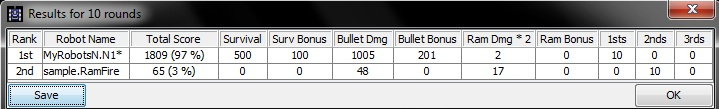
\includegraphics[width=\textwidth]{n1-ramfire.jpg}
\end{figure}

\begin{figure}[h!]
  \caption{N1 vs. Crazy statistics}
  \centering
    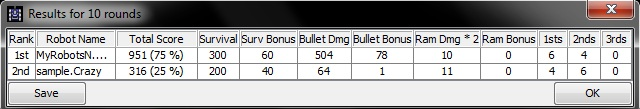
\includegraphics[width=\textwidth]{n1-crazy.jpg}
\end{figure}



\subsection{Helena - Model-based reflex agent}

Helena is a peaceful robot.\footnote{Word \textit{robot} was first used
in play R.U.R. by Czech interwar playwright Karel Čapek. Helena is a name of a
fictional robot character in this play, a robot who develops human feelings.}
This robot waits until attacked by enemy and then applies a counter-strategy
based on perceptions of attacker's behaviour.

After homing to the middle of the battlefield, Helena scans the battlefield and
waits. She keeps track of how many times she was rammed by another robot and how
many bullets hit her. This is her \textbf{model} of the environment - keeping
track of those two variables helps Helena to decide which strategy to use
against the enemy. Every time a bullet hits her or another robot rams her, she
resolves whether she is using the right strategy (and changes it eventually),
by comparing those two variables.

Since behaviour of RamFire robot is easily recognizable (ramming exceeds firing)
and his movements easily predictable (going to the last known location if
scanned enemy so it can ram it), counter-strategy for beating RamFire robot was
created in design-time and Helena just needs to follow it. Helena is going
backwards for 200 px, firing one bullet and then turning 90\degree~. Enemy
RamFire robots receives the bullet, scans Helena and drives to her location.
Before he arrives there, the pattern repeats: Helena is 200 px off the side of
the enemy, shoots at him, turns and escapes again and again.

\begin{figure}[h!]
  \caption{Helena vs. RamFire statistics}
  \centering
    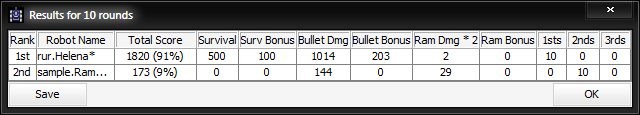
\includegraphics[width=\textwidth]{helena-ramfire.png}
\end{figure}

Robot called Crazy, on the other hand, moves through the battlefield following
crazy patterns (hence it's name probably), and it is unpredictable, where is he
going to and what his next actions could be like. Applying on him the same
counter-strategy as on RamFire would not be reasonable and Helena applies a
different one. This strategy is does not beat Crazy and is implemented just for
illustration of different strategies.

\begin{figure}[h!]
  \caption{Helena vs. Crazy statistics}
  \centering
    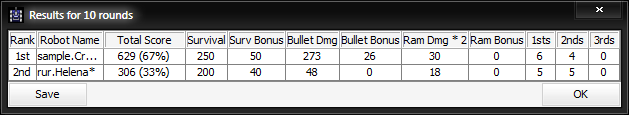
\includegraphics[width=\textwidth]{helena-crazy.png}
\end{figure}

\end{document}
